%%%%%%%%%%%%%%%%%%%%%%%%%%%%%%%%%%%%%%%%%%%%%%%%%%%%%%%%%%
\documentclass[xcolor=pdftex,dvipsnames,table,10pt]{beamer}
%handout, if no \pause

\usepackage{tabularx}
\usepackage[]{algorithm2e}
\usepackage{listings}
\usepackage{lstautogobble}

%\documentclass[handout,xcolor=pdftex,dvipsnames,table]{beamer} % USE THIS WITH pdfpages STUFF
%\usepackage{pgfpages}
%\pgfpagesuselayout{resize to}[a4paper, landscape]

\definecolor{headerColour}{RGB}{180, 230, 245}
\definecolor{headerTitleColour}{RGB}{0, 60, 80}
\definecolor{sectionShadedColour}{RGB}{50, 110, 130}
\definecolor{subsectionHighlightColour}{RGB}{50, 50, 50}
\definecolor{subsectionShadedColour}{RGB}{100, 100, 100}

\setbeamercolor{subsection in sidebar}{fg=subsectionHighlightColour}
\setbeamercolor{subsection in sidebar shaded}{fg=subsectionShadedColour}
\setbeamercolor{structure}{fg=headerTitleColour, bg=headerColour}
\setbeamercolor{title}{fg=headerTitleColour, bg=white}
\setbeamercolor{section in sidebar shaded}{fg=sectionShadedColour}

\usetheme{Goettingen}
\makeatletter\setbeamertemplate{sidebar canvas \beamer@sidebarside}[vertical shading][top=headerColour,bottom=white]\makeatother

%% to suppress subsections in sidebar:
%\setbeamertemplate{subsection in sidebar shaded}
%{\vspace*{-\baselineskip}}
%\setbeamertemplate{subsubsection in sidebar shaded}
%{\vspace*{-\baselineskip}}

\usepackage{amsmath, amssymb}
\usepackage{fancyvrb}


% Font modification
\usefonttheme{professionalfonts}
\usepackage{cmbright}
\usepackage{eulervm}
\newfont{\Ss}{cmcsc12 scaled 1600}

% no navigation symbols at the bottom of frames
\beamertemplatenavigationsymbolsempty
\setbeamertemplate{footline}[frame number] 

\usepackage{multirow} % allows entries across multipe rows in tables
\usepackage{booktabs} % makes fancier rulers in tables
%\usepackage{setspace} % spacing between lines

%%%%%%%%%%%%%%%%%%
%% Bibliography related stuff:
% control space between lines
  \let\oldthebibliography=\thebibliography
  \let\endoldthebibliography=\endthebibliography
  \renewenvironment{thebibliography}[1]{
    \begin{oldthebibliography}{#1}
      \setlength{\parskip}{-0.5ex}
      \setlength{\itemsep}{-0.5ex}
  }{ \end{oldthebibliography} }
% Force entry to be in one line
\setbeamertemplate{bibliography entry title}{}
\setbeamertemplate{bibliography entry location}{}
\setbeamertemplate{bibliography entry note}{}
% Set bullet point shape:
\setbeamertemplate{bibliography item}{-}
%%%%%%%%%%%%%%


\newenvironment{items}{\begin{list}{$\bullet$}{\itemsep0ex plus 0.2ex
\parsep0ex plus 0.2ex \topsep0ex \parskip0ex}}{\end{list}}
\newcommand{\head}[1]
{\slide{\begin{center}\textbf{#1}\vspace*{-0.5\baselineskip}
{\color{red}\rule{\textwidth}{1mm}}\end{center}}}
\parskip0.3ex

\newcommand{\cT}{{\mathcal T}}


%\defbeamertemplate*{title page}{customized}[1][]
%{
%  \titlepage
%  \usebeamerfont{title}\inserttitle\par
%  \usebeamerfont{subtitle}\usebeamercolor[fg]{subtitle}\insertsubtitle\par
%  \bigskip
%  \usebeamerfont{author}\insertauthor\par
%  \usebeamerfont{institute}\insertinstitute\par
%  \usebeamerfont{date}\insertdate\par
%  \usebeamercolor[fg]{titlegraphic}\inserttitlegraphic
%}



\author[]{Lecturers: \\ Tanja Stadler \& Carsten Magnus \& Alexei Drummond \\ \bigskip Teaching Assistants: \\  Veronika Bo\v{s}kov\'{a} \& J\={u}lija Pe\v{c}erska}
\institute{Computational Evolution \\ Department of Biosystems Science and Engineering}
\title[MEPP]{Molecular Evolution, \\ Phylogenetics \& Phylodynamics} 
\date{HS 2015}
\titlegraphic{\hspace*{8cm}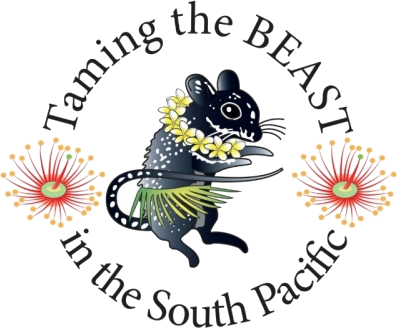
\includegraphics[height=1.5cm]{figures/TTBSP_logo.png}}
%{\small Link to Script\&Slides:  \url{http://www.tb.ethz.ch/education} 
%}

%%%%%%%%%%%%%% Figure caption setup
\usepackage[compatibility=false]{caption}
\captionsetup[figure]{labelsep=space,justification=centering}
\renewcommand{\figurename}{\scriptsize Figure adapted from}

% syntax: \figureCaption{Citation caption}{Second (real) caption}
% second caption can be skipped, first one has to be suppressed if you want to skip it
\newcommand\figureCaption[2]{%
  \captionsetup{aboveskip=0.1cm,belowskip=0cm}
  \caption{\scriptsize #1}
  \caption*{#2}
}

%%%%%%%%%%%%%% Fixme and comment setup§
\definecolor{red}{HTML}{C92D39}
\definecolor{green}{HTML}{498A44}

% syntax: \fixme{What needs to be fixed}
\newcommand{\fixme}[1]{\textcolor{red}{\texttt{{\bf FIX ME:} #1}}}
% Hide all fixmes by switching the line above to this:
%\newcommand{\fixme}[1]{}

% syntax: \comment{Name of commenter}{C omment}
\newcommand{\comment}[2]{\textcolor{green}{{\bf Comment by {#1}}: #2}}
% Hide all comments by switching the line above to this:
%\newcommand{\comment}[2]{}

\definecolor{correct}{HTML}{025B0A}
\definecolor{incorrect}{gray}{0.6}

\newenvironment{questions}{
	\begin{enumerate}[1)]
		\setlength{\itemsep}{1cm}
		\setlength{\parskip}{-0.1cm}
}{\end{enumerate}}

\newenvironment{answers}{
	\begin{enumerate}[a)]
		\setlength{\itemsep}{0cm}
		\setlength{\topsep}{0cm}
		\setlength{\parskip}{0cm}
		\setlength{\parsep}{0cm}
}{\end{enumerate}}

\begin{document}

\begin{frame}
  \titlepage
\end{frame}

\section{TITLE}

%%%%%%%%%%%%%%%%%%%%%%%%%%%%%%%%%%%%%%%%%%%%%%%%%%%%%%%%%%
%%%%%%%%%%%%%%%%%%%%outline%%%%%%%%%%%%%%%%%%%%%%
%%%%%%%%%%%%%%%%%%%%%%%%%%%%%%%%%%%%%%%%%%%%%%%%%%%%%%%%%%
\begin{frame}\frametitle{Outline of lecture xx}
  \begin{itemize}
   \item EXAMPLE1
    \begin{itemize}
    \item[-] EXAMPLE1.1
    \item[-] EXAMPLE2.1
    \end{itemize}
  \end{itemize}
  \begin{itemize}  
   \item EXAMPLE2
    \begin{itemize}
    \item[-] EXAMPLE2.1
    \item[-] EXAMPLE2.2
    \end{itemize}
  \end{itemize}
\end{frame}

\subsection{EXAMPLE1}

\begin{frame}\frametitle{Sample frame, both captions}
  \begin{figure}[h!]
    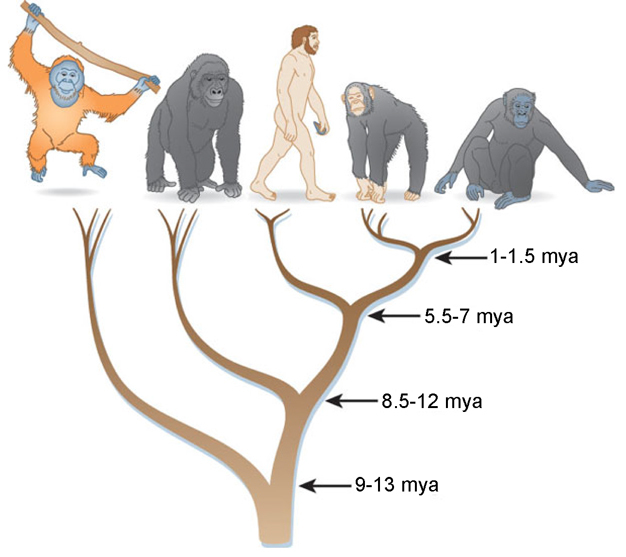
\includegraphics[height=5cm]{figures/TS-Apes.jpg}
	\figureCaption{\cite{Paabo2003}}{This is a tree. We can tell it's a tree because it has some branches. And we'll have a very long label to match it.}
  \end{figure}
\end{frame}

\begin{frame}\frametitle{Sample frame, no first caption}
  \begin{figure}[h!]
    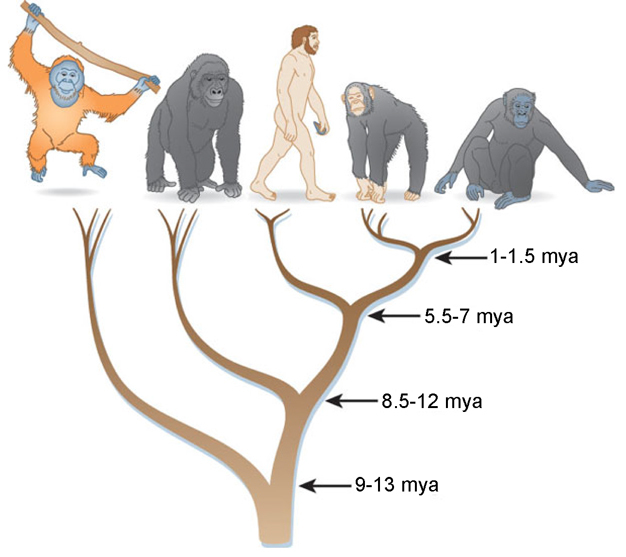
\includegraphics[height=5cm]{figures/TS-Apes.jpg}
    \def\figurename{}
	\figureCaption{}{This is a tree. We can tell it's a tree because it has some branches. And we'll have a very long label to match it.}
  \end{figure}
  We skipped the first, reference caption here.
\end{frame}

\begin{frame}\frametitle{Sample frame, no second caption}
  \begin{figure}[h!]
    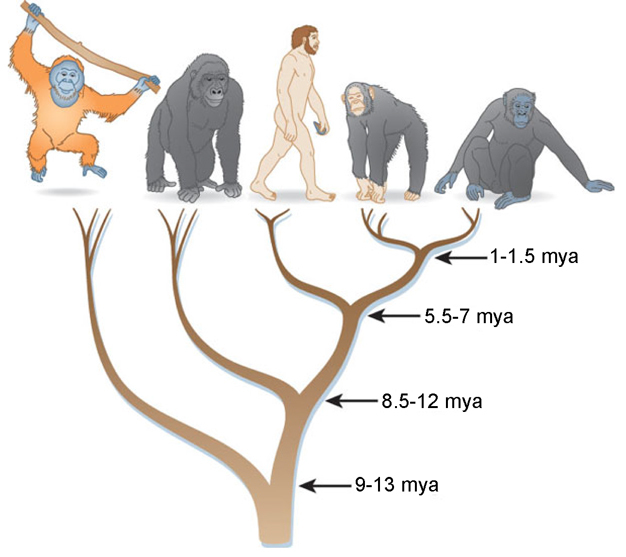
\includegraphics[height=5cm]{figures/TS-Apes.jpg}
	\figureCaption{\cite{Paabo2003}}{}
  \end{figure}
  We skipped the second caption here.
\end{frame}

\begin{frame}\frametitle{Sample frame, side-by-side list and figure}
  \begin{columns}[t]
  \column{0.65\linewidth}
    \begin{itemize}
      \item DNA (Deoxyribonucleic acid) first isolated by Friedrich Miescher\\ (born in Basel in 1844; Institute here in Basel named after him)
      \item DNA is a double helix\\ (published by Watson \& Crick in 1953 in Nature; based on images by Rosalind Franklin; Nobel price in 1962)
    \end{itemize}
  \column{0.35\linewidth}
    \begin{figure}[h!]
      
\includegraphics[width=0.5\textwidth]{figures/TS-DNA1953.pdf}
      \figureCaption{\cite{Watson1953}}{This is a DNA helix, imagine that.}
    \end{figure}
  \end{columns} 
\end{frame}

\begin{frame}\frametitle{Sample frame, a fixme and a comment}
    \fixme{Oh no, some stuff needs fixing!}
    
    \comment{J\=ulija}{This requires attention!}
\end{frame}

\section{References}
\begin{frame}[t,allowframebreaks]\frametitle{References}
\bibliographystyle{apalike}
\tiny\bibliography{bibliography}
\end{frame}

\end{document}
